% abtex2-modelo-artigo.tex, v-1.9.2 laurocesar
% Copyright 2012-2014 by abnTeX2 group at http://abntex2.googlecode.com/ 
%

% ------------------------------------------------------------------------
% ------------------------------------------------------------------------
% abnTeX2: Modelo de Artigo Acadêmico em conformidade com
% ABNT NBR 6022:2003: Informação e documentação - Artigo em publicação 
% periódica científica impressa - Apresentação
% ------------------------------------------------------------------------
% ------------------------------------------------------------------------

\documentclass[
	% -- opções da classe memoir --
	article,			% indica que é um artigo acadêmico
	11pt,				% tamanho da fonte
	oneside,			% para impressão apenas no verso. Oposto a twoside
	a4paper,			% tamanho do papel. 
	% -- opções da classe abntex2 --
	%chapter=TITLE,		% títulos de capítulos convertidos em letras maiúsculas
	%section=TITLE,		% títulos de seções convertidos em letras maiúsculas
	%subsection=TITLE,	% títulos de subseções convertidos em letras maiúsculas
	%subsubsection=TITLE % títulos de subsubseções convertidos em letras maiúsculas
	% -- opções do pacote babel --
	english,			% idioma adicional para hifenização
	brazil,				% o último idioma é o principal do documento
	sumario=tradicional
	]{abntex2}


% ---
% PACOTES
% ---

% ---
% Pacotes fundamentais 
% ---
\usepackage{lmodern}			% Usa a fonte Latin Modern
\usepackage[T1]{fontenc}		% Selecao de codigos de fonte.
\usepackage[utf8]{inputenc}		% Codificacao do documento (conversão automática dos acentos)
\usepackage{indentfirst}		% Indenta o primeiro parágrafo de cada seção.
\usepackage{nomencl} 			% Lista de simbolos
\usepackage{color}				% Controle das cores
\usepackage{graphicx}			% Inclusão de gráficos
\usepackage{microtype} 			% para melhorias de justificação
\usepackage{float}
% ---
		
% ---
% Pacotes adicionais, usados apenas no âmbito do Modelo Canônico do abnteX2
% ---
\usepackage{lipsum}				% para geração de dummy text
% ---
		
% ---
% Pacotes de citações
% ---
\usepackage[brazilian,hyperpageref]{backref}	 % Paginas com as citações na bibl
\usepackage[alf]{abntex2cite}	% Citações padrão ABNT
% ---

% ---
% Configurações do pacote backref
% Usado sem a opção hyperpageref de backref
\renewcommand{\backrefpagesname}{Citado na(s) página(s):~}
% Texto padrão antes do número das páginas
\renewcommand{\backref}{}
% Define os textos da citação
\renewcommand*{\backrefalt}[4]{
	\ifcase #1 %
		Nenhuma citação no texto.%
	\or
		Citado na página #2.%
	\else
		Citado #1 vezes nas páginas #2.%
	\fi}%
% ---

% ---
% Informações de dados para CAPA e FOLHA DE ROSTO
% ---
\titulo{Linguagens, Autômatos e Computação\\ Avaliação Individual 2}
\author{Ramiro Berneira Nascimento\thanks{ramirobnascimento@hotmail.com}}
\local{Brasil}
\data{2021, 02 de julho}
% ---

% ---
% Configurações de aparência do PDF final

% alterando o aspecto da cor azul
\definecolor{blue}{RGB}{41,5,195}

% informações do PDF
\makeatletter
\hypersetup{
     	%pagebackref=true,
		pdftitle={\@title}, 
		pdfauthor={\@author},
    	pdfsubject={Modelo de artigo científico com abnTeX2},
	    pdfcreator={LaTeX with abnTeX2},
		pdfkeywords={abnt}{latex}{abntex}{abntex2}{atigo científico}, 
		colorlinks=true,       		% false: boxed links; true: colored links
    	linkcolor=blue,          	% color of internal links
    	citecolor=blue,        		% color of links to bibliography
    	filecolor=magenta,      		% color of file links
		urlcolor=blue,
		bookmarksdepth=4
}
\makeatother
% --- 

% ---
% compila o indice
% ---
\makeindex
% ---

% ---
% Altera as margens padrões
% ---
\setlrmarginsandblock{3cm}{3cm}{*}
\setulmarginsandblock{3cm}{3cm}{*}
\checkandfixthelayout
% ---

% --- 
% Espaçamentos entre linhas e parágrafos 
% --- 

% O tamanho do parágrafo é dado por:
\setlength{\parindent}{1.3cm}

% Controle do espaçamento entre um parágrafo e outro:
\setlength{\parskip}{0.2cm}  % tente também \onelineskip

% Espaçamento simples
\SingleSpacing

% ----
% Início do documento
% ----
\begin{document}

% Retira espaço extra obsoleto entre as frases.
\frenchspacing 

% ----------------------------------------------------------
% ELEMENTOS PRÉ-TEXTUAIS
% ----------------------------------------------------------

%---
%
% Se desejar escrever o artigo em duas colunas, descomente a linha abaixo
% e a linha com o texto ``FIM DE ARTIGO EM DUAS COLUNAS''.
% \twocolumn[    		% INICIO DE ARTIGO EM DUAS COLUNAS
%
%---
% página de titulo
\maketitle
% resumo em português
\begin{resumoumacoluna}
     Este artigo científico foi proposto como a Atividade Avaliativa Individual Final da cadeira de Linguagens, Autômatos e Computação ministrada pelo professor Diego Vrague Noble, no primeiro semestre de 2021 no curso de Engenharia de Software da Universidade PUCRS. O objetivo principal desta atividade foi desenvolver o conhecimento dos seguintes tópicos, Máquina de Turing Universal e Gramática Regular.
 
 \vspace{\onelineskip}
 
 \noindent
 \textbf{Palavras-chaves}: Máquina de Turing Universal. Gramática Regular.
\end{resumoumacoluna}

% ]  				% FIM DE ARTIGO EM DUAS COLUNAS
% ---

% ----------------------------------------------------------
% ELEMENTOS TEXTUAIS
% ----------------------------------------------------------
\textual

% ----------------------------------------------------------
% Introdução
% ----------------------------------------------------------
\section*{Introdução}
\addcontentsline{toc}{section}{Introdução}

    Neste artigo, serão aprofundados e dissertados dois tópicos distintos. Máquina de Turing Universal e a resolução de um problema envolvendo Gramática Regular.  
    
    Para que se possa entender e definir uma Máquina de Turing Universal, será necessário abordar outros sub-tópicos primeiro, como a definição de uma Máquina de Turing, qual a importância da definição desta maquina para a computação, com quais elementos uma Máquina de Turing é definida e como ela opera. Com este conjunto de elementos, esta máquina lê os símbolos de uma posição da fita, decide o que vai escrever nesta posição e para qual lado a fita será movida para repetir o processo. Durante esse processo, o estado Q da máquina vai mudando até chegar, ou não, a um estado final, definindo a palavra de entrada (valores da fita) como um programa aprovado ou rejeitado.
    
    O segundo problema proposto nesta avaliação é a solução do seguinte problema:
    
    Uma Gramática Regular (GR) é uma gramática onde todas as regras são da forma $A → aB$ ou $A → b$ onde A e B são variáveis quaisquer e a e b são terminais quaisquer. O conjunto de linguagens geradas por GRs é o conjunto de linguagens regulares. Portanto, qualquer GR pode ser convertida em um Autômato Finito Não-Determinístico (AFND) que aceita a  mesma linguagem gerada pela GR. Dada GR abaixo, converta-a para um AFND que aceite a mesma linguagem e explique os passos feitos na forma de um algoritmo:
    
    $G = ({A,B}, {a,b,c,d}, R, A)$ a relação R é definida pelas seguintes produções:
    
                             \[A \longrightarrow aB | aA\] 
                            \[B \longrightarrow bB | aA | cA | d\]
                            
    

% ----------------------------------------------------------
% Seção de explicações
% ----------------------------------------------------------
\section{Máquina de Turing Universal}

    Alan Turing foi um matemático britânico que estava em busca da prova matemática de que o problema proposto por David Hilbert e Wilhelm Ackermann, o \textbf{Entscheidungsproblem}, nao tinha um método ou procedimento geral efetivo para calcular ou computar todas as instancias do problema.\citeonline{wiki_turing_machine}

    
    A partir desse objetivo, Turing criou, o que ele próprio chamava na época, de Máquina Computável (hoje conhecida como Máquina de Turing), composta de uma fita com infinitas células, um cabeçote de leitura e escrita, e um controle configurável que computa e permite mover o cabeçote 1 célula para a esquerda ou para direita. Para programar esta máquina foi definido conjunto de 7 elementos, conhecido como \textbf{Tupla} que juntos são capazes definir uma Máquina de Turing e reconhecer ou não uma determinada entrada a partir desta configuração da máquina. Em uma comparação simples com o que temos nos dias atuais, uma Máquina de Turing seria equivalente a um programa de um computador digital moderno. Em outras palavras, é um algoritmo que recebe valores de entrada que segue um conjunto pré-determinado de passos que gera um resultado previsível e determinístico. 
    
    A definição formal e teórica de uma Máquina de Turing de apenas uma fita é composta da seguinte Tupla:
    
    \begin{itemize}
        \item $\Sigma$: um alfabeto finito de entrada (não contém o símbolo branco)
        \item Q: um conjunto finito de estados
        \item $\delta$: conjunto de funções de transição
        \item $\Gamma$: é o alfabeto da fita
        \item $Q_0 \in Q$: estado inicial
        \item $Q_{final} \in Q $: conjunto de estados de aceitação
        \item $Q_{rejeita} \in Q $: conjunto de estados de rejeição
\end{itemize}
    
    Com este conjunto de elementos, esta máquina lê os símbolos de uma posição da fita, decide o que vai escrever nesta posição e para qual lado a fita será movida para repetir o processo. Durante esse processo, o estado Q da máquina vai mudando até chegar ou não a um estado final, tornando a palavra de entrada (valores da fita), um programa reconhecido ou não reconhecido. 
    
    Turing, entendendo essa ideia, foi um passo além e imaginou uma máquina maior e mais dominante que pudesse controlar a entrada e a saída dessas máquinas computáveis que haviam dentro dela.  Chamada de máquina universal ou \textbf{Máquina de Turing Universal}, esse sistema seria composta de uma ou mais Máquinas de Turing dentro dela, podendo operacionalizar as entradas das sub-maquina e armazenar as suas saída. Este conceito foi teoricamente comprovado e futuramente definido como \textbf{Arquitetura de von Neumann}, que até hoje é considerado como o conceito teórico de qualquer computador moderno. 
    
    \subsection{Operando uma Máquina de Turing com uma fita}
    Antes de entendermos como uma máquina de Turing Universal funciona, temos que ter um entendimento básico de como uma máquina de Turing funciona. Uma máquina de Turing opera utilizando os 7 itens da Tupla em conjunto para definir a entrada, a computação e a saída.
    
    A entrada de uma Máquina de Turing é definida pelo conjunto de entrada $\Sigma$ e o estado inicial $Q_0$ que ditam o que vai ser escrito na fita e qual o estado inicial da máquina.  O conjunto de entrada, é escrito desde a posição zero da fita até $n$ elementos, sendo $n$ o tamanho do conjunto $\Sigma$. A posição $n+1$ da fita contém um símbolo branco $b$ que corresponde ao fim do conjunto de elementos $\Sigma$. 
    
	A configuração da máquina, que em outras palavras significa o que a máquina irá computar para gerar a saída, é composta pelo conjunto das funções de transição $\delta$ e o conjunto finito de estados $Q$. Em cada função de transição $\delta$ é definido as seguintes ações no momento da leitura:
	
    	[${\delta : Q\times \Gamma } \longrightarrow  Q\times \Gamma \times {\leftarrow ,\rightarrow}$]
    	
    \begin{itemize}
        \item 1º $Q = $ em que estado $Q$ a máquina está;
        \item 1º $\Gamma$ = o que o cabeçote deve estar lendo;
        
        $\longrightarrow$
        
        \item 2º $Q = $ para que estado a máquina irá;
		\item 2º $\Gamma$ = o que deve ser escrito naquela célula da fita;
		\item ${\leftarrow ,\rightarrow}$ = para que lado que a fita irá correr 1 célula.
			
	\end{itemize}
	
    O conjunto destas funções de transições compõem os movimentos possíveis dentro do autômato, levando o resultado para uma sequencia de estados $Q$ interligados por estas funções. Na Figura \ref{fig:funcao_de_transicao} podemos ver a relação entre esses 2 elementos da Tupla e entender melhor como seria o interior teórico de uma Maquina de Turing.
        
\begin{figure}
\centering
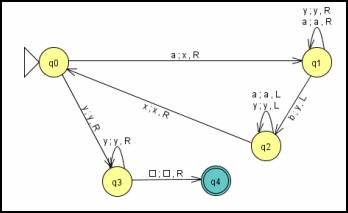
\includegraphics[width=0.5\textwidth]{funcao_de_transicao.jpg}
\caption{\label{fig:funcao_de_transicao}Funções de transição em um conjunto de estados.}
\end{figure}

    E finalizando o processo da Máquina, após definir os símbolos iniciais da fita, definindo o estado inicial e seguindo os passos configurados nas funções de transição que levam a um estado $Q$, a máquina gera um resultado que pode colocar o autômato em estado um destes dois estados: \textbf{\textit{reconhecimento} ou \textit{aceitação}} ou  \textbf{\textit{não-reconhecimento} ou \textit{rejeição}}. 


\subsection{Como funciona uma Maquina de Turing Universal}
    Compreendendo o que é uma Máquina de Turing, podemos subir esta ideia mais um nível e criar uma outra Máquina de Turing, chamada de U, para testar, configurar e escrever os dados de entrada em uma secundária Máquina de Turing. 
    
    O principal objetivo da Máquina de Turing Universal $U$ é simular uma outra sub Máquina de Turing $M$ para entender se, a partir de uma String de entrada $w$ em $M$, é possível dizer se $w$ é aceita, rejeitada ou se entra em laço em $M$.
    
    \[A_{TM} = {<M,w> |  \frac{M\text{ é uma Maquina de Turing}}
                              {w\text{ palavra aceita por M} }} \]
    
    A máquina $U$ tem como entrada as configurações codificadas de $M$ em uma palavra e uma outra palavra de \textit{input} $w$. Após a execução, a Máquina $U$ determina se a Máquina $M$ em $w$ é aceita, rejeitada ou entre em laço infinito. Caso entre em laço, dizemos que não é decidível.
    
\section{Problema da Gramática Regular}
    Como segunda tarefa desta atividade avaliativa, foi proposta que, a partir de uma Gramática Regular passada pelo professor, a mesma fosse convertida para um Automato Finito Não-Determinístico e que explicássemos quais foram os passos para chegar em tal resultado. 
    
\subsection{O Problema}
    Os dados da Gramática Regular(GR) foram passadas através do que define uma GR de forma formal. Através dos dados da 4-upla $G = (V,T,R,S)$, equivalentes a:
    \begin{itemize}
        \item G = a própria Gramatica Regular
        \item V = conjunto finito de Variáveis
        \item T = conjunto finito, disjunto de V, denominado Terminais
        \item R = conjunto finito de regras, onde cada regra é uma Variável e uma cadeia de variáveis Terminais
        \item S = a Variável inicial
    \end{itemize}
    
    A proposta do exercício nos concebe a seguinte 4-upla:
    $G = (\{A,B\}, \{a,b,c,d\}, R, A)$, sendo R =
        \[A \rightarrow aB | aA\]
\[B \rightarrow bB | aA | cA | d\]
    
    
    Tendo a definição da nossa GR, já podemos dar inicio ao processo de conversão de Gramática Regular em um Automato Finito Não-Determinístico utilizando o Algoritmo de Thompson.
\subsection{Algoritmo de Thompson}
    O Algoritmo de Thompson tem como finalidade transformar uma Expressão Regular em um Automato Finito Não-Determinístico. O que normalmente se pensa ao entender este algoritmo é: mas se eles são equivalentes e tem como transformar um no outro, por que fazer esta conversão? qual seria a finalidade de transformar uma GR em um AFND e vice-versa?  \citeonline{wiki_thompson_algorithm}
    
    Na computação, GR e ER são muito utilizadas em algoritmos de processamento de texto, como a biblioteca Pattern do Java 8. Já, os autômatos, são mais utilizados em compiladores e em nível de máquina. No final das contas, ambos representam a mesma coisa, porém em formatos diferentes. Isso nos mostra, também, que ambas representações fazem parte do mesmo grupo, das \textbf{Linguagens Regulares}.
    
    A maneira como o algoritmo faz para transformar uma GR em um AFND é muito interessante. São uma sequencia de passos que vão aos poucos convertendo um monte de regras da Gramatica Regular nos estados dos Autômatos.
    
    \begin{enumerate}
        \item Gramatica Regular $\rightarrow$ Expressão Regular
        \item Expressão Regular $\rightarrow$ Sub-expressões Regulares Constituintes
        \item Sub-expressões Regulares Constituintes $\rightarrow$ Autômatos
    \end{enumerate}
    
    Entendendo agora o passo a passo, podemos aplicar para o nosso caso:
    
\subsubsection{Algoritmo}
\cite{dca_conversao_gr_afnd}
    Dada a nossa Gramatica Regular $G = (\{A,B\}, \{a,b,c,d\}, R, A)$ precisamos, primeiramente convertê-la para uma expressão regular. Para isso, devemos ver o conjunto de regras e por qual variável a gramática começa e então escrever a lógica. Convertendo, chegamos a este resultado:
    
                        \[ ER = ((a+)((((a|c)(a+))*|(b+))*)d) \]
                        
                        
    Tendo nossa ER em mãos, podemos agora fragmentá-la em sub-expressões para criar o autômato em partes. Para isso devemos pegar cada operação e dividir na menor parte possível, para então, transformar cada pedaço em um autômato. Como exemplo, pegamos a primeira operação atômica da nossa ER, o $a$ e separamos ele do resto, tornando-o a Sub-expressão1($S_e1$). Tendo essa sub-expressão, criamos o autômato pra ele e subimos um nível de complexidade, unindo a $S_e1$ com a operação de quantificação criando o $a+$, correspondente a sub-expressão $S_e2$. Replicamos ao resto das sub-expressões regulares, até que tenhamos o autômato completo no final da etapa:
    
    \begin{itemize}
        \item $S_e1$ = a 
            \begin{figure}[H]
\centering
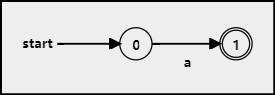
\includegraphics[width=0.5\textwidth]{r1.jpg}
\caption{\label{fig:r1} Autômato referente a $S_e1$.}
\
\end{figure}
        \item $S_e2$ = a+ 
            \begin{figure}[H]
\centering
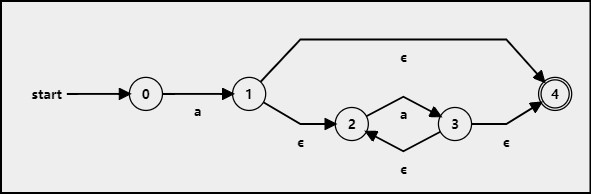
\includegraphics[width=0.5\textwidth]{r2.jpg}
\caption{\label{fig:r2}Autômato referente a $S_e2$.}
\end{figure}
        \item $S_e3$ = c 
            \begin{figure}[H]
\centering
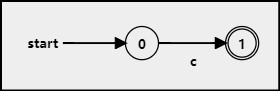
\includegraphics[width=0.5\textwidth]{r3.jpg}
\caption{\label{fig:r3}Autômato referente a $S_e3$.}
\end{figure}
        \item $S_e4$ = $S_e1|S_e3$ 
            \begin{figure}[H]
\centering
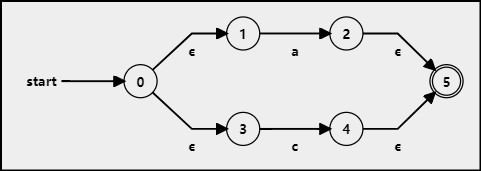
\includegraphics[width=0.5\textwidth]{r4.jpg}
\caption{\label{fig:r4}Autômato referente a $S_e4$.}
\end{figure}
        \item $S_e5$ = $S_e4S_e2$ 
            \begin{figure}[H]
\centering
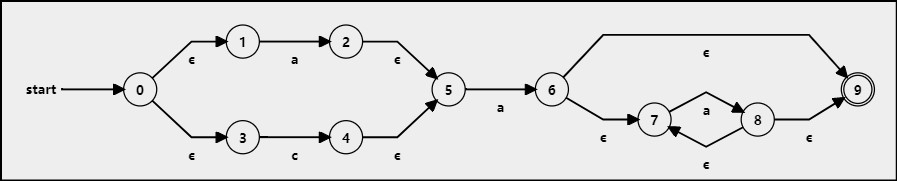
\includegraphics[width=0.5\textwidth]{r5.jpg}
\caption{\label{fig:r5}Autômato referente a $S_e5$.}
\end{figure}
        \item $S_e6$ = $S_e5*$ 
            \begin{figure}[H]
\centering
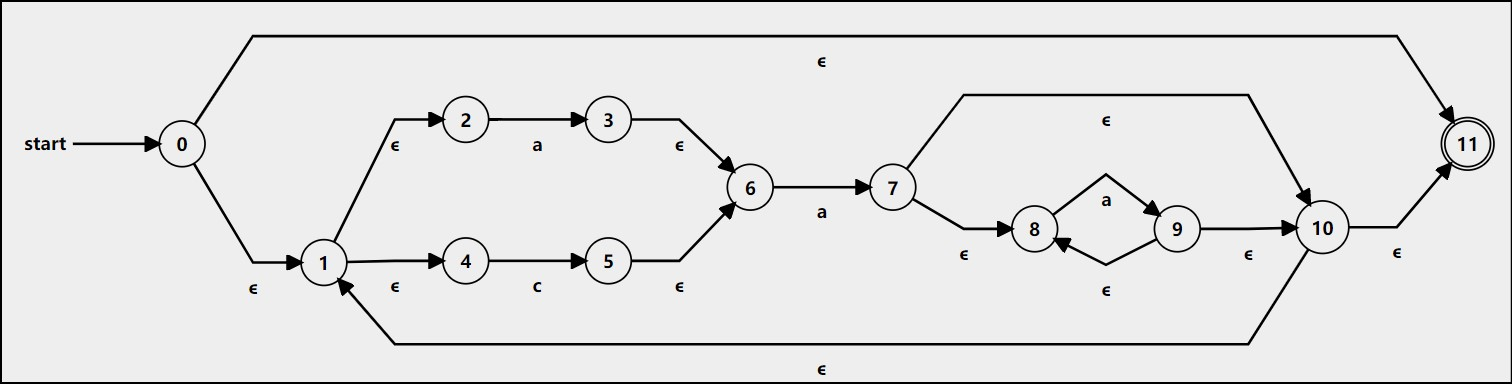
\includegraphics[width=0.5\textwidth]{r6.jpg}
\caption{\label{fig:r6}Autômato referente a $S_e6$.}
\end{figure}
        \item $S_e7$ = b+ 
            \begin{figure}[H]
\centering
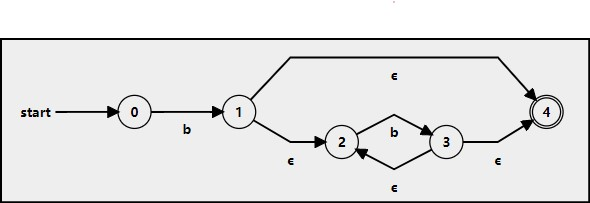
\includegraphics[width=0.5\textwidth]{r7.jpg}
\caption{\label{fig:r7}Autômato referente a $S_e7$.}
\end{figure}
        \item $S_e8$ = $S_e6|S_e7$ 
            \begin{figure}[H]
\centering
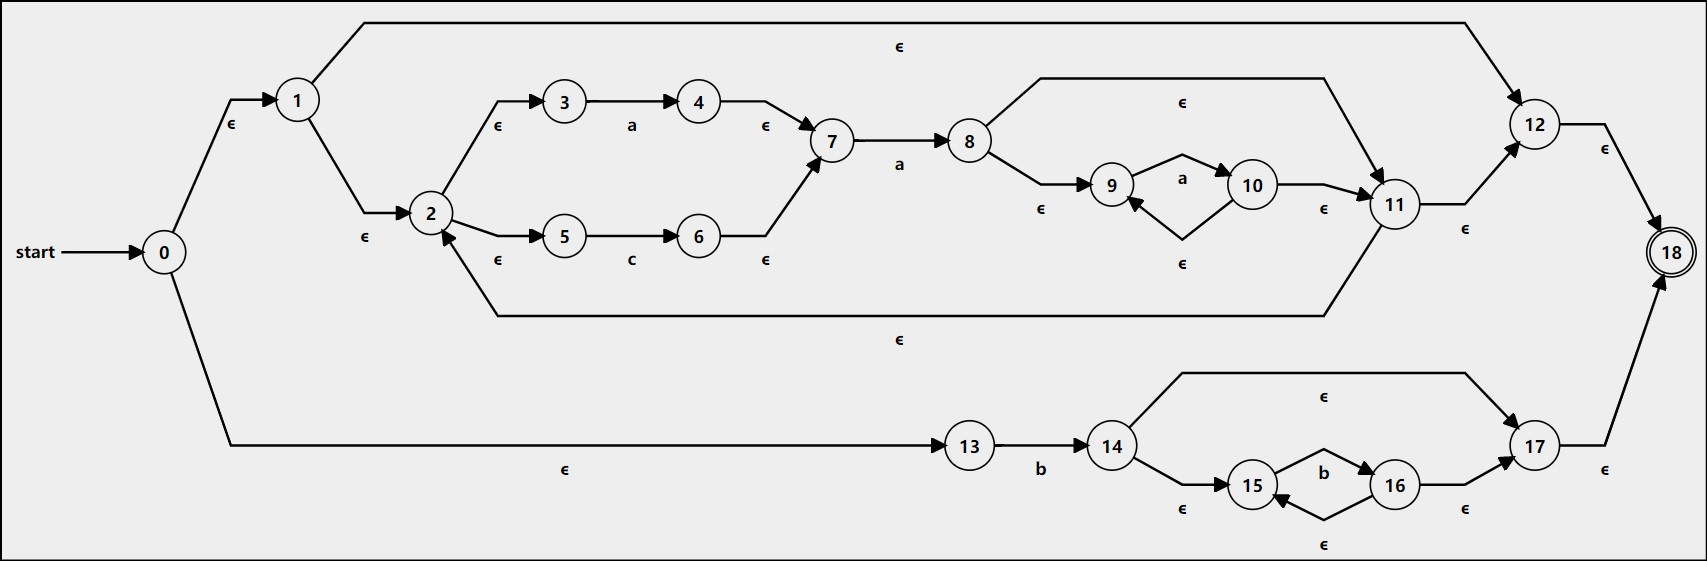
\includegraphics[width=0.5\textwidth]{r8.jpg}
\caption{\label{fig:r8}Autômato referente a $S_e8$.}
\end{figure}
        \item $S_e9$ = $S_e8*$ 
            \begin{figure}[H]
\centering
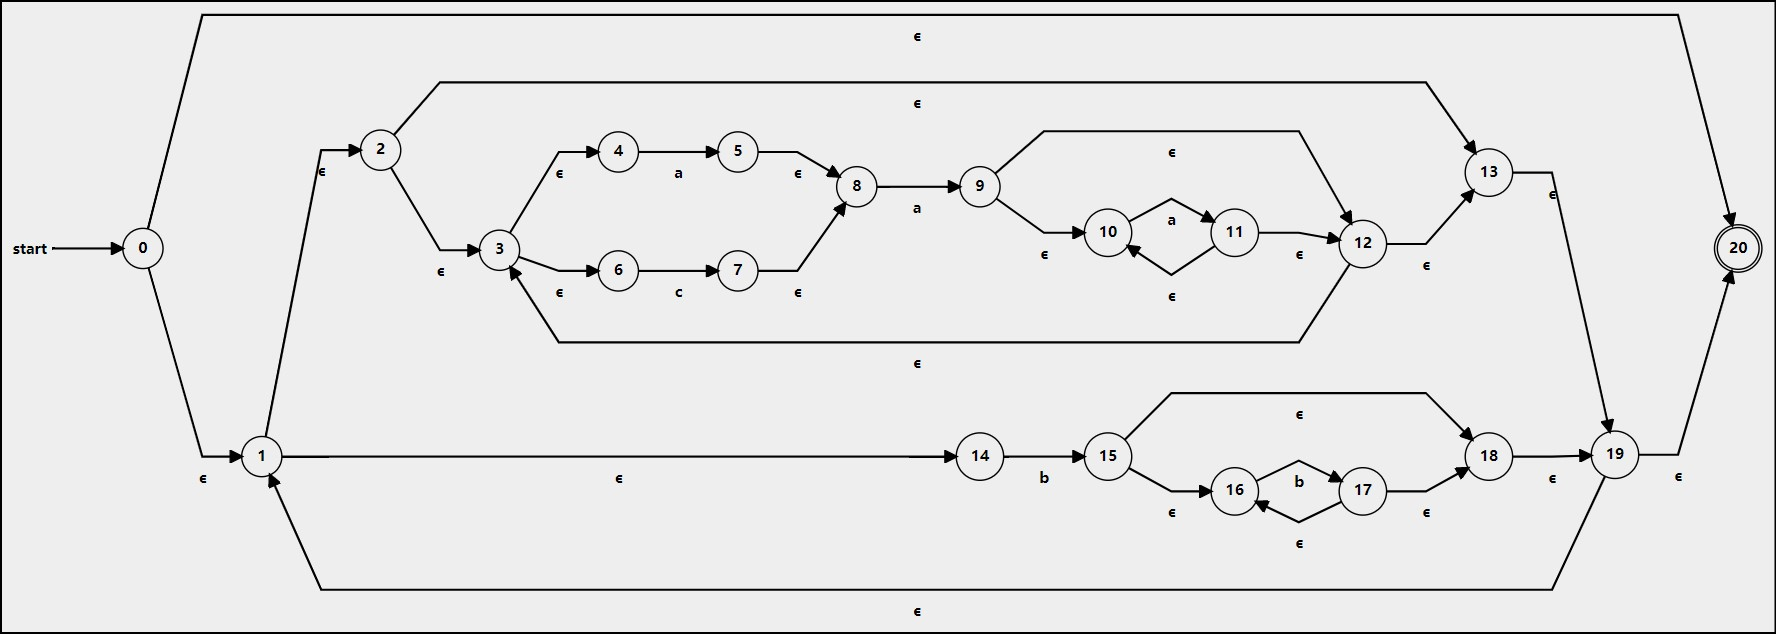
\includegraphics[width=0.5\textwidth]{r9.jpg}
\caption{\label{fig:r9}Autômato referente a $S_e9$.}
\end{figure}
        \item $S_e10$ = d 
            \begin{figure}[H]
\centering
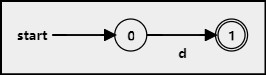
\includegraphics[width=0.5\textwidth]{r10.jpg}
\caption{\label{fig:r10}Autômato referente a $S_e10$.}
\end{figure}
        \item $S_e11$ = $S_e2S_e9S_e10$ 
            \begin{figure}[H]
\centering
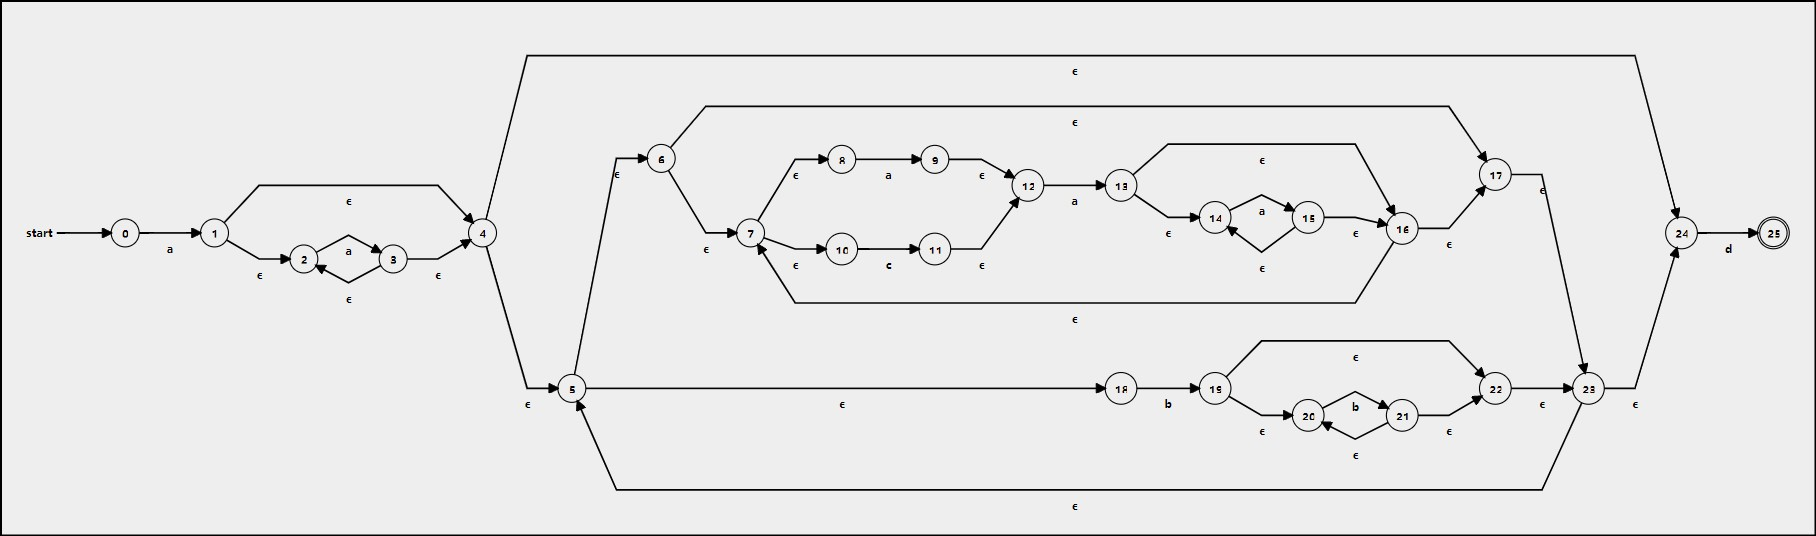
\includegraphics[width=0.5\textwidth]{r11.jpg}
\caption{\label{fig:r11}Autômato referente a $S_e11$.}
\end{figure}
    \end{itemize}
    
    Assim, em $S_e11$, temos a conversão final que nos gera a representação final do que era inicialmente uma Gramática Regular em um Autômato Finito Não-Determinístico. 
    
    %\bibliographystyle{alpha}
    %\bibliography{sample}

\section*{Considerações finais}
\addcontentsline{toc}{section}{Considerações finais}
    A elaboração desta atividade foi excelente para apurar os conhecimentos abordados ao longo da cadeira. Estudando e pesquisando sobre a Máquina de Turing Universal, trouxeram o aprofundamento de conceitos vistos no início do semestre, como autômatos, e o quão presente o conceito da Máquina de Turing está nos dias de hoje. Também, entender o que ela pode e não pode fazer, é um conceito essencial para o desenvolvimento profissional na aréa da Tecnologia da Informação.
    
    Já a proposta do segundo desafio foi muito proveitoso, pois dispertou em mim a pergunta "por que precismos desta conversão?". Solucionando este problema de conversão da Gramática Regular para AFND, me fez entender a aplicabilidade no mundo real de cada uma dessas formas de Linguagens Regulares.

% ----------------------------------------------------------
% ELEMENTOS PÓS-TEXTUAIS
% ----------------------------------------------------------
\postextual

% ---
% Título e resumo em língua estrangeira
% ---

% \twocolumn[    		% INICIO DE ARTIGO EM DUAS COLUNAS

% titulo em inglês
\titulo{Linguagens, Autômatos e Computação\\ Avaliação Individual 2}
\emptythanks
\maketitle

% resumo em português
\renewcommand{\resumoname}{Abstract}
\begin{resumoumacoluna}
 \begin{otherlanguage*}{english}
   This scientific paper was proposed as the Final Individual Assessment Activity from the Languages, Automates and Computation class ministered by professor Diego Vrague Noble, at the first semester of 2021 of Software Engineering in PUCRS University. The main goal of this activity is develop the knowledge of the following topics, Universal Turing Machine and Regular Grammar.  

   \vspace{\onelineskip}
 
   \noindent
   \textbf{Key-words}: Universal Turing Machine. Regular Grammar.
 \end{otherlanguage*}  
\end{resumoumacoluna}

% ]  				% FIM DE ARTIGO EM DUAS COLUNAS
% ---

% ----------------------------------------------------------
% Referências bibliográficas
% ----------------------------------------------------------
\bibliography{abntex2-modelo-references}




% ----------------------------------------------------------
% Glossário
% ----------------------------------------------------------
%
% Há diversas soluções prontas para glossário em LaTeX. 
% Consulte o manual do abnTeX2 para obter sugestões.
%
%\glossary

% ----------------------------------------------------------
% Apêndices
% ----------------------------------------------------------

% ---
% Inicia os apêndices
% ---

% ---

% ----------------------------------------------------------
% Anexos
% ----------------------------------------------------------
% ---
% Inicia os anexos
% ---
%\anexos


\end{document}
